%versi 2 (8-10-2016)
\chapter{Kuesioner Untuk Umpan Balik}
\label{lamp:A}

\def\scl{1}
% \def\leg{\legend{Switching,Homotopic,Buffer*Length,Length}}
\def\leg{} 
\def\std{none}
\def\ymin{}
\def\ymax{}

Kuesioner yang disebarkan beserta dengan responnya untuk mendapatkan umpan balik bagi yang menguji coba aplikasi IDE UNPAR mobile.

\begin{figure}[H] 
	\centering  
	\centering
	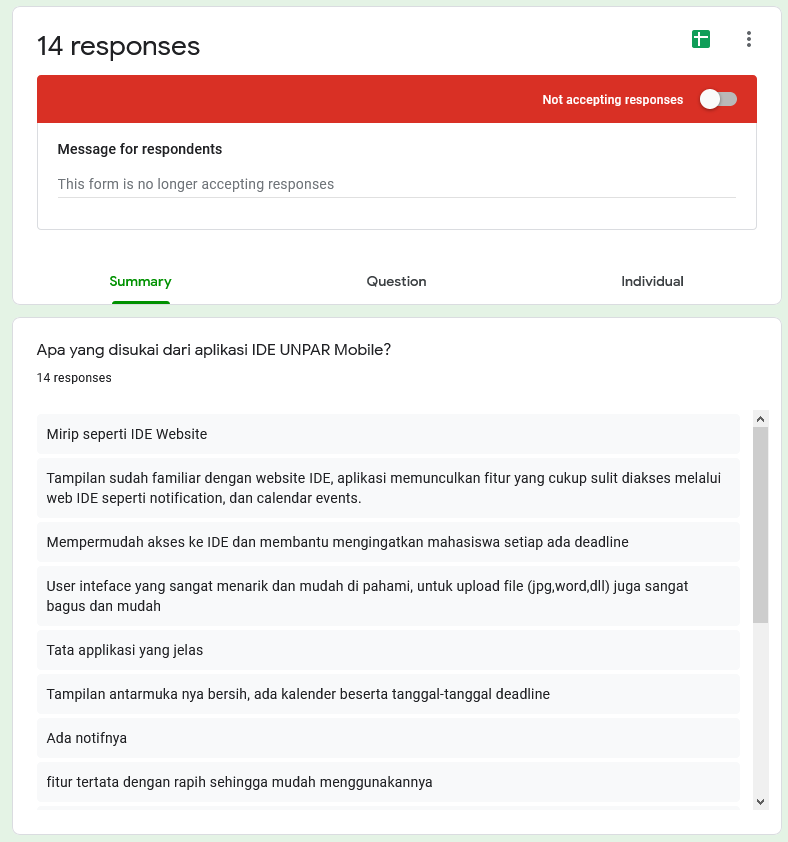
\includegraphics[scale=0.6]{form-questionaire-1.png}
	\caption{\textit{Header} dan pertanyaan pertama}
	\label{fig:questionaire} 
\end{figure} 

\begin{figure}
	\centering
	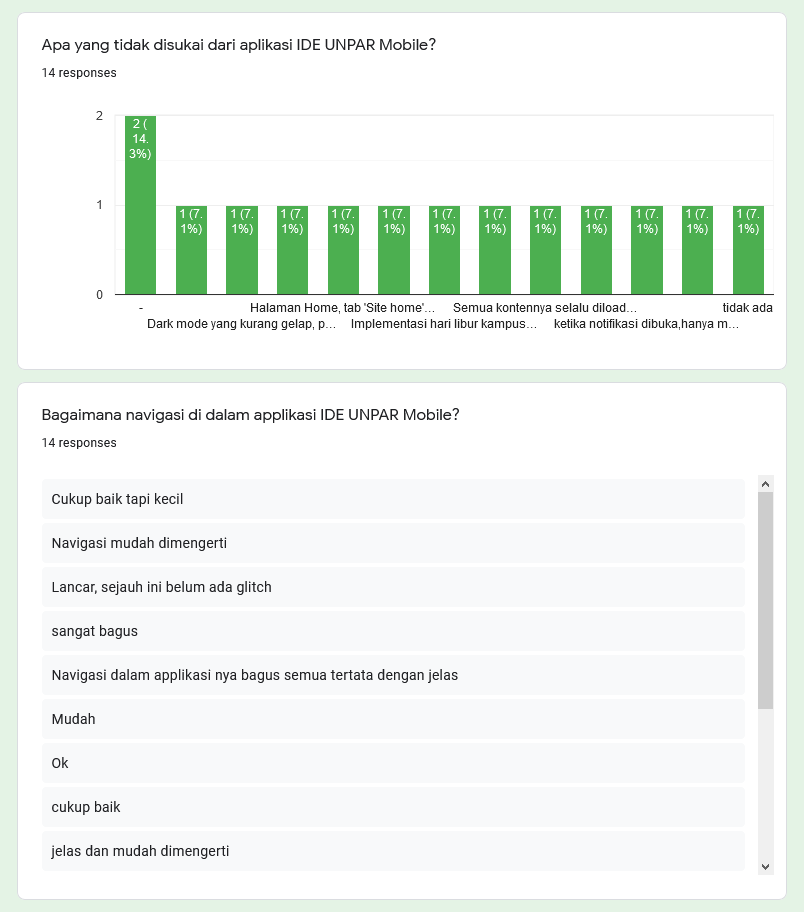
\includegraphics[scale=0.6]{form-questionaire-2.png}
	\caption{Pertanyaan kedua dan ketiga}
\end{figure}

\begin{figure}
	\centering
	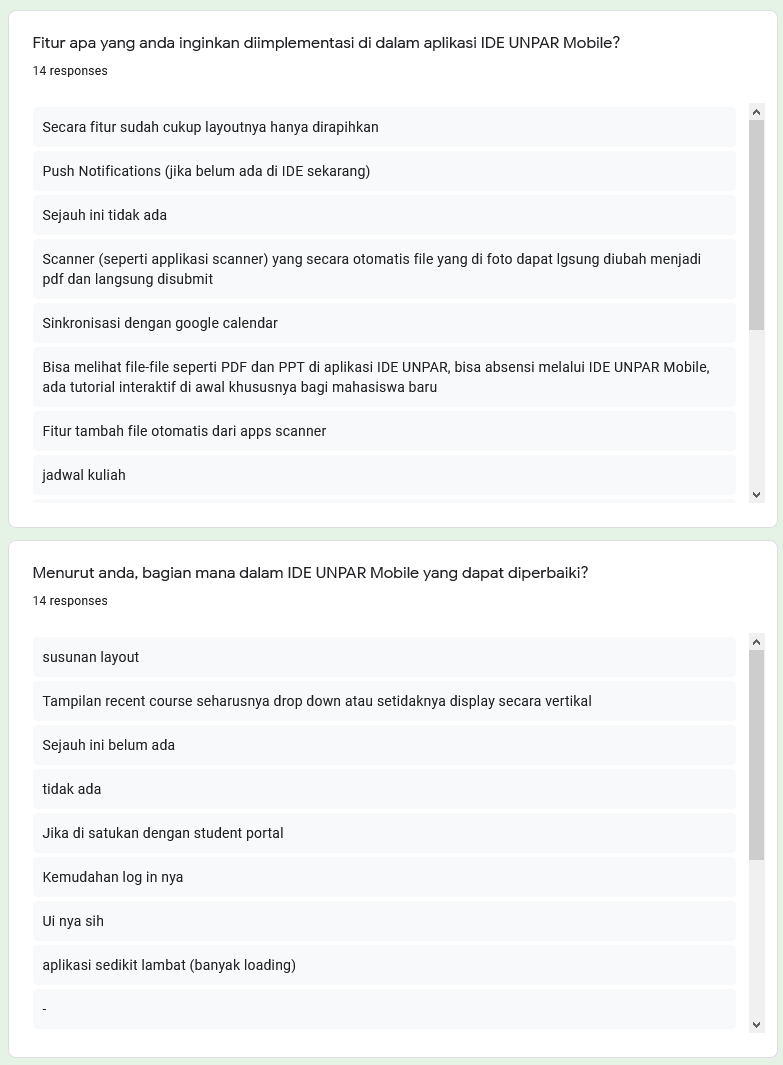
\includegraphics[scale=0.6]{form-questionaire-3.png}
	\caption{Pertanyaan keempat dan kelima}
\end{figure}